\section{Group Evaporative Coolers}\label{group-evaporative-coolers}

This group of objects describes the properties and configuration for the evaporative coolers models for the HVAC section.

\subsection{EvaporativeCooler:Direct:CelDekPad}\label{evaporativecoolerdirectceldekpad}

The direct stage, shown in the figure below, consists of a rigid media evaporative pad, with water recirculated from a reservoir. The water is pumped from the reservoir to a water distribution header, for water feed by gravity from above the media. The evaporative pad provides the area for the adiabatic saturation of the air. While the process provides a lower dry-bulb temperature, the moisture content of the leaving air is higher than the entering condition. The direct stage is used for comfort cooling in a building where adding humidity to the air can be tolerated.

\begin{figure}[hbtp] % fig 144
\centering

\includegraphics[width=0.9\textwidth, height=0.9\textheight, keepaspectratio=true]{media/image415.png}
\caption{Direct Stage Evaporative Cooler \protect \label{fig:direct-stage-evaporative-cooler}}
\end{figure}

The thermodynamic process is a simultaneous heat and mass transfer, or adiabatic cooling, and follows a constant enthalpy line on the psychrometric chart, it is shown in the figure below as a process from A to B. Since the deviation of the constant wet-bulb line and the constant enthalpy line is small, it is assumed that the wet-bulb temperature is constant across the direct evaporative stage.

\begin{figure}[hbtp] % fig 145
\centering
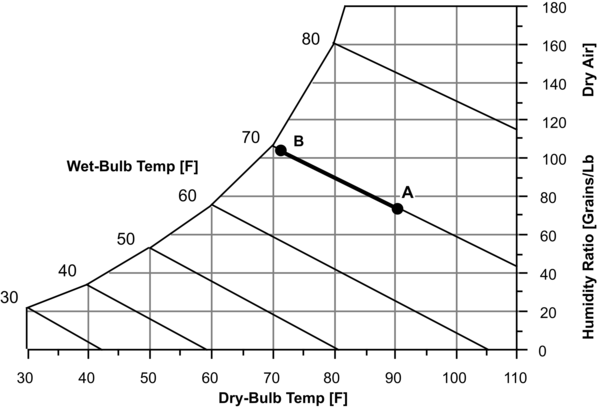
\includegraphics[width=0.9\textwidth, height=0.9\textheight, keepaspectratio=true]{media/image416.png}
\caption{Psychrometric Chart -- Constant Enthalpy \protect \label{fig:psychrometric-chart-constant-enthalpy}}
\end{figure}

If the direct evaporative process were 100\% efficient, the leaving dry-bulb temperature would equal the entering wet-bulb temperature. The efficiency of the direct evaporative process is less than 100\% and by defining saturation efficiency (\(\varepsilon\) se) for the direct stage or evaporative pad, the leaving dry-bulb temperature can be expressed by the following equation.

\begin{equation}
{T_{db\,supout}} = {T_{db\,sup\,in}} - {\varepsilon_{se}}\cdot \left( {{T_{db\,sup\,in}} - {T_{wb\,sup\,in}}} \right)
\end{equation}

\subsubsection{Inputs}\label{inputs-016}

\paragraph{Field: Name}\label{field-name-015}

A unique identifying name for each evaporative cooler.

\paragraph{Field:Availability Schedule Name}\label{fieldavailability-schedule-name}

The name of a schedule which defines when the evaporative cooler is available. A schedule value of 0 indicates that the evaporative cooler is off for that time period. A schedule value greater than 0 indicates that the evaporative cooler can operate during the time period. If this field is blank, the schedule has values of 1 for all time periods.

\paragraph{Field: Direct Pad Area}\label{field-direct-pad-area}

The face area of the evaporative pad in m\(^{2}\). With the area and mass flow rate, the air velocity is calculated and is used to determine the saturation efficiency. This field is autosizable.

\paragraph{Field: Direct Pad Depth}\label{field-direct-pad-depth}

The depth of the evaporative pad in meters. The pad depth is used to determine the saturation efficiency. This field is autosizable.

\paragraph{Field: Recirculating Water Pump Power Consumption}\label{field-recirculating-water-pump-power-consumption}

This field is used to specify the power consumed by the evaporative cooler recirculating pump in Watts.

\paragraph{Field: Air Inlet Node Name}\label{field-air-inlet-node-name-001}

The name of the evaporative cooler air inlet node from the Air Loop Simulation.

\paragraph{Field: Air Outlet Node Name}\label{field-air-outlet-node-name-001}

The name of the evaporative cooler air outlet node from the Air Loop Simulation.

\paragraph{Field: Control Type}\label{field-control-type-001}

This input field is currently unused and can be left blank.

\paragraph{Field: Water Supply Storage Tank Name}\label{field-water-supply-storage-tank-name-000}

This field is optional. It is used to describe where the cooler obtains water used for evaporative cooling. If blank or omitted, then the cooler will obtain water directly from the mains. If the name of a WaterUse:Storage object is used here, then the cooler will obtain its water from that tank. If a tank is specified, the cooler will attempt to obtain all the water it uses from the tank. However if the tank cannot provide all the water the cooler needs, then the cooler will still operate and obtain the rest of the water it needs from the mains.

An IDF example showing how this object is:

\begin{lstlisting}

EvaporativeCooler:Direct:CelDekPad,
  Evaporative Cooler,           !- Name
  System Availability Schedule,   !- Availability Schedule Name
  0.6,                                         !- Direct Pad Area {m2}
  0.2,                                         !- Direct Pad Depth {m}
  225,                                         !- Recirculating Water Pump Power Consumption {W}
  Evap Cooler Inlet Node,   !- Air Inlet Node Name
  Supply Outlet Node;           !- Air Outlet Node Name
\end{lstlisting}

\subsubsection{Outputs}\label{outputs-011}

The output variables that are available for this direct evaporative cooler are shown below:

\begin{itemize}
\item
  HVAC,Average, Evaporative Cooler Wet Bulb Effectiveness
\item
  HVAC,Average, Evaporative Cooler Electric Power{[}W{]}
\item
  HVAC,Sum, Evaporative Cooler Electric Energy {[}J{]}
\item
  HVAC,Sum, Evaporative Cooler Water Volume{[}m3{]}
\item
  HVAC,Sum,Evaporative Cooler Mains Water Volume {[}m3{]}
\item
  HVAC,Sum,Evaporative Cooler Storage Tank Water Volume {[}m3{]}
\item
  HVAC,Sum,Evaporative Cooler Starved Water Volume {[}m3{]}
\item
  HVAC,Sum,Evaporative Cooler Starved Mains Water Volume {[}m3{]}
\end{itemize}

\paragraph{Evaporative Cooler Wet Bulb Effectiveness}\label{evaporative-cooler-wet-bulb-effectiveness}

The effectivenss, or saturation efficiency, is the temperature change of the supply air divided by the difference between the inlet air dry-bulb and wet-bulb temperatures. In other words, it is a measure of the approach to the inlet air wet-bulb temperature.

\paragraph{Evaporative Cooler Electric Power{[}W{]}}\label{evaporative-cooler-electric-powerw}

\paragraph{Evaporative Cooler Electric Energy {[}J{]}}\label{evaporative-cooler-electric-energy-j}

These output variables report the electric power and electric energy required to operate the water pump.

\paragraph{Evaporative Cooler Water Volume {[}m3{]}}\label{evaporative-cooler-water-volume-m3}

The water consumption is the water evaporated from the pad. This water consumption is only from the direct thermodynamics of water evaporation and does not include other sources of consumption such as drift or concentration blow down. This output variable appears when mains water is supplied to the cooler.

\paragraph{Evaporative Cooler Mains Water Volume {[}m3{]}}\label{evaporative-cooler-mains-water-volume-m3}

This is the source of the water consumed. This output variable appears when mains water is supplied to the cooler.

\paragraph{Evaporative Cooler Storage Tank Water Volume {[}m3{]}}\label{evaporative-cooler-storage-tank-water-volume-m3}

The water consumption is the water evaporated from the pad. This water consumption is only from the direct thermodynamics of water evaporation and does not include other sources of consumption such as drift or concentration blow down. This output variable appears when storage tank water is supplied to the cooler.

\paragraph{Evaporative Cooler Starved Water Volume {[}m3{]}}\label{evaporative-cooler-starved-water-volume-m3}

This is the water consumed by the evaporative cooler that could not accually be met by the storage tank. This output variable appears when storage tank water is supplied to the cooler.

\paragraph{Evaporative Cooler Starved Mains Water Volume {[}m3{]}}\label{evaporative-cooler-starved-mains-water-volume-m3}

This is the source (mains) of water consumed by the evaporative cooler that could not accually be met by the storage tank. This output variable appears when storage tank water is supplied to the cooler.

\subsection{EvaporativeCooler:Direct:ResearchSpecial}\label{evaporativecoolerdirectresearchspecial}

This cooler is similar in principal to the EvaporativeCooler:Direct:CelDekPad. The model differs in that it gives the user a simple way of specify the cooler effectiveness. Using the ResearchSpecial input object also allows the cooler to control the amount of cooling based on node setpoints (controlled by SetpointManagers). This avoid problems from over cooling when conditions are such that loads are low and cooling power is high.

The model allows to vary the effectiveness depending on the primary air flow rates. The design effectiveness is modified by multiplying with Effectiveness Flow Fraction Modifier Curve value. The flow fraction is the ratio of the current primary airflow rate to the design flow rate. The recirculating and spray water pump power is assumed to vary with the primary air flow. The design pump power is modified using user specified pump modifier curve value. The normalized pump power modifier curve is a function of primary air flow fraction as a independent variable.

Also the direct evaporative cooler operating range can be controlled depending on the entering air dry bulb and wet bulb temperatures. The operating range controlled based on minimum and maximum inlet node air temperature limits. The evaporative cooler can be turned on or off depending user specified minimum and maximum temperature limits. If the inlet node entering air temperature is lower or higher than the minimum and maximum limits, respectively, then the direct research special evaporative cooler is turned off. If these two input fields are left blank then, no user specified operating temperature control is applied. Operating range control feature is primarily intended for application in data centers.

\subsubsection{Inputs}\label{inputs-1-014}

\paragraph{Field: Name}\label{field-name-1-013}

A unique identifying name for each cooler.

\paragraph{Field: Availability Schedule Name}\label{field-availability-schedule-name-006}

The name of a schedule that defines when the evaporative cooler is available. A schedule value of 0 indicates that the evaporative cooler is off for that time period. A schedule value greater than 0 indicates that the evaporative cooler can operate during the time period. If this field is blank, the schedule has values of 1 for all time periods.

\paragraph{Field: Cooler Design Effectiveness}\label{field-cooler-design-effectiveness}

This field specifies the effectiveness at design flow rate that is applied to the wetbulb depression to determine the conditions leaving the cooler. This model assumes that the effectiveness can vary with supply air flow rate. For effectiveness variation with supply air flow fraction enter the Effectiveness Flow Ratio Modifier Curve Name input field below. The flow fraction is the ratio of the sum of current primary air and secondary air sides flow rates and the sum of the design flow rates.

\paragraph{Field: Effectiveness Flow Ratio Modifier Curve Name}\label{field-effectiveness-flow-ratio-modifier-curve-name}

This curve modifies the effectiveness design value specified the previous field by multiplying the value by the result of this curve. The modifying curve is a function of flow fraction, which is the ratio of the current primary air flow rates divided by the design primary air flow rates. If this input field is left blank, the effectiveness is assumed to be constant. Any curve or table with one independent variable can be used. Any curve or table with one independent variable can be used: Curve:Linear, Curve:Quadratic, Curve:Cubic, Curve:Quartic, Curve:Exponent, Curve:ExponentialSkewNormal, Curve:Sigmoid, Curve:RectuangularHyperbola1, Curve:RectangularHyperbola2, Curve:ExponentialDecay, Curve:DoubleExponentialDecay, and Table:OneIndependentVariable.

\paragraph{Field:Primary Design Air Flow Rate}\label{fieldprimary-design-air-flow-rate}

This numeric input field is the primary air design air flow rate in m3/s. This input field is autosizable. If the evaporative cooler is on main air loop branch, the design flow rate is the same as branch design flow rate, or else if it is on outdoor air system it will be the maximum of the the outdoor air design flow rate and the half of the primary air flow rate on the main air loop branch.

\paragraph{Field: Recirculationg Water Pump Design Power}\label{field-recirculationg-water-pump-design-power}

This numeric input field is the recirculating and spray pump electric power at Secondary Design Air Flow Rate in W. This is the nominal water recirculating and spray pump power of evaporative cooler at primary air design flow rates and cooler design effectiveness. This input field is autosizable. Average Pump Power sizing factor was estimated from pump power and primary air design flow rates inputs from energyplus example files is about 90.0 {[}W/(m3/s){]} ( = 90.0 \textasciitilde{} Pump Power / Primary Air Design Flow Rate). The factor ranges from 55.0 to 150.0 {[}W/(m3/s){]}.

\paragraph{Field: Water Pump Power Sizing Factor}\label{field-water-pump-power-sizing-factor}

This numeric input field value is recirculating water pump sizing factor in W/(m3/s). This field is used when the previous field is set to autosize. The pump design electric power is scaled with Secondary Design Air Flow Rate. This input field is autosizable. Average Pump Power sizing factor was estimated from pump power and primary air design flow rates inputs from energyplus example files is about 90.0 {[}W/(m3/s){]} ( = 90.0 \textasciitilde{} Pump Power / Primary Air Design Flow Rate). The factor ranges from 55.0 to 150.0 {[}W/(m3/s){]}.

\paragraph{Field: Water Pump Power Modifier Curve Name}\label{field-water-pump-power-modifier-curve-name}

This alpha input field is the name of a dimensionless normalized pump power modifying curve. This curve modifies the pump electric power in the previous field by multiplying the design power by the result of this curve. The normalized curve is a function of the primary air flow fraction as independent variable. The curve shall yield a value of 1.0 at a flow fraction of 1.0. The flow fraction is the ratio of the primary air during current operation divided by primary air Design Air Flow Rate. If this input field is left blank, the pump power is assumed to lineary vary with the load. Any curve or table with one independent variable can be used: Curve:Linear, Curve:Quadratic, Curve:Cubic, Curve:Quartic, Curve:Exponent, Curve:ExponentialSkewNormal, Curve:Sigmoid, Curve:RectuangularHyperbola1, Curve:RectangularHyperbola2, Curve:ExponentialDecay, Curve:DoubleExponentialDecay, and Table:OneIndependentVariable.

\paragraph{Field: Air Inlet Node Name}\label{field-air-inlet-node-name-1-001}

The name of the air inlet node for the primary air flow path through the cooler.

\paragraph{Field: Air Outlet Node Name}\label{field-air-outlet-node-name-1-000}

The name of the air outlet node for the primary air flow path through the cooler.

\paragraph{Field: Sensor Node Name}\label{field-sensor-node-name-001}

This field specifies the name of a node that will provide system air temperature setpoint information. A separate SetpointManager object should be setup to update this node.

\paragraph{Field: Water Supply Storage Tank Name}\label{field-water-supply-storage-tank-name-1}

This field is optional. It is used to describe where the cooler obtains water used for evaporative cooling. If blank or omitted, then the cooler will obtain water directly from the mains. If the name of a WaterUse:Storage object is used here, then the cooler will obtain its water from that tank. If a tank is specified, the cooler will attempt to obtain all the water it uses from the tank. However, if the tank cannot provide all the water the cooler needs, then the cooler will still operate and obtain the rest of the water it needs from the mains.

\paragraph{Field: Drift Loss Fraction}\label{field-drift-loss-fraction}

This field is optional and can be used to model additional water consumed by the cooler from drift. Drift is water that leaves the cooling media as droplets and does not evaporate into the process air stream. For example, water may get blown off the evaporative media by winds and escape the air system. The value entered here is a simple fraction of the water consumed by the cooler for normal process evaporation. The amount of drift is this fraction times the water evaporated for the normal cooling process. This field can be left blank and then there will be no added water consumption from drift.

\paragraph{Field: Blowdown Concentration Ratio}\label{field-blowdown-concentration-ratio-000}

This field is optional and can be used to model additional water consumed by the cooler from blowdown. Blowdown is water that is intentionally drained from the cooler s sump to offset the build up of solids in the water that would otherwise occur because of evaporation. The value entered here is dimensionless. It can be characterized as the ratio of solids in the blowdown water to solids in the make up water. Typical values are 3 to 5. The default is 3.0.

\paragraph{Field: Evaporative Cooler Operation Minimum Drybulb Temperature}\label{field-evaporative-cooler-operation-minimum-drybulb-temperature}

This numeric field defines the evaporative cooler inlet node drybulb temperature minimum limit in degrees Celsius. The evaporative cooler will be turned off when evaporator cooler air inlet node dry-bulb temperature falls below this value. The typical minimum value is 16 °C. Users are allowed to specify their own limits. If this field is left blank, then there is no drybulb temperature lower limit for evaporative cooler operation.

\paragraph{Field: Evaporative Operation Maximum Limit Wetbulb Temperature}\label{field-evaporative-operation-maximum-limit-wetbulb-temperature}

This numeric field defines the evaporative cooler air inlet node air wetbulb temperature maximum limits in degree Celsius. When the evaporative cooler air inlet node air wetbulb temperature exceeds this limit, then the evaporative cooler is turns off. The typical maximum value is 24 °C. If this input field is left blank, then there is no wetbulb temperature upper limit for evaporative cooler operation.

\paragraph{Field: Evaporative Operation Maximum Limit Drybulb Temperature}\label{field-evaporative-operation-maximum-limit-drybulb-temperature}

This numeric field defines the evaporative cooler air inlet node drybulb temperature maximum limits in degree Celsius. The evaporative cooler will be turned off when the evaporative cooler air inlet node drybulb temperature exceeds this value. The typical maximum value is 28 °C. If this input field is left blank, then there is no upper drybulb temperature limit for evaporative cooler operation.

An example IDF entry is

\begin{lstlisting}

EvaporativeCooler:Direct:ResearchSpecial,
  Direct Evap Cooler, !- Name
  ALWAYS_ON, !- Availability Schedule Name
  0.7 , !- Cooler Design Effectiveness
  ,     !- Effectiveness Flow Ratio Modifier Curve Name
  30.0 , !- Recirculating Water Pump Design Power
  ,     !- Water Pump Power Sizing Factor
  ,     !- Water Pump Power Modifier Curve Name
  OAIndRDD Evap Cooler- OADirect Evap CoolerNode , !- Air Inlet Node Name
  OADirect Evap Cooler- OAMixing BoxNode, !- Air Outlet Node Name
  OADirect Evap Cooler- OAMixing BoxNode, !- Sensor Node Name
  , !- Water Supply Storage Tank Name
  0.0, !- Drift Loss Fraction
  3; !- Blowdown Concentration Ratio
\end{lstlisting}

\subsubsection{Outputs}\label{outputs-1-009}

The output variables that are available for this direct evaporative cooler are shown below:

\begin{itemize}
\item
  HVAC,Average, Evaporative Cooler Electric Power{[}W{]}
\item
  HVAC,Average, Evaporative Cooler Stage Effectiveness {[]}
\item
  HVAC,Sum, Evaporative Cooler Electric Energy {[}J{]}
\item
  HVAC,Sum, Evaporative Cooler Water Volume{[}m3{]}
\item
  HVAC,Sum,Evaporative Cooler Mains Water Volume {[}m3{]}
\item
  HVAC,Sum,Evaporative Cooler Storage Tank Water Volume {[}m3{]}
\item
  HVAC,Sum,Evaporative Cooler Starved Water Volume {[}m3{]}
\item
  HVAC,Sum,Evaporative Cooler Starved Mains Water Volume {[}m3{]}
\end{itemize}

\paragraph{Evaporative Cooler Electric Power{[}W{]}}\label{evaporative-cooler-electric-powerw-1}

\paragraph{Evaporative Cooler Electric Energy {[}J{]}}\label{evaporative-cooler-electric-energy-j-1}

These output variables report the electric power and electric energy required to operate the water pump.

\paragraph{Evaporative Cooler Stage Effectiveness {[]}}\label{evaporative-cooler-stage-effectiveness}

The cooler stage efficiency is defined as the temperature change of the supply air divided by the difference between the outdoor dry-bulb and wet-bulb temperatures, including the effect of the reduction in the primary air flow rate in other words, it is a measure of the approach to the entering air wet-bulb temperature.

\paragraph{Evaporative Cooler Water Volume {[}m3{]}}\label{evaporative-cooler-water-volume-m3-1}

The water consumption is the water evaporated from the pad. This water consumption is only from the direct thermodynamics of water evaporation and does not include other sources of consumption such as drift or concentration blow down. This output variable appears when mains water is supplied to the cooler.

\paragraph{Evaporative Cooler Mains Water Volume {[}m3{]}}\label{evaporative-cooler-mains-water-volume-m3-1}

This is the source of the water consumed. This output variable appears when mains water is supplied to the cooler.

\paragraph{Evaporative Cooler Storage Tank Water Volume {[}m3{]}}\label{evaporative-cooler-storage-tank-water-volume-m3-1}

The water consumption is the water evaporated from the pad. This water consumption is only from the direct thermodynamics of water evaporation and does not include other sources of consumption such as drift or concentration blow down. This output variable appears when storage tank water is supplied to the cooler.

\paragraph{Evaporative Cooler Starved Water Volume {[}m3{]}}\label{evaporative-cooler-starved-water-volume-m3-1}

This is the water consumed by the evaporative cooler that could not accually be met by the storage tank. This output variable appears when storage tank water is supplied to the cooler.

\paragraph{Evaporative Cooler Starved Mains Water Volume {[}m3{]}}\label{evaporative-cooler-starved-mains-water-volume-m3-1}

This is the source (mains) of water consumed by the evaporative cooler that could not accually be met by the storage tank. This output variable appears when storage tank water is supplied to the cooler.

\subsection{EvaporativeCooler:Indirect:CelDekPad}\label{evaporativecoolerindirectceldekpad}

The dry coil indirect evaporative cooler, shown in the figure below, has a rigid media pad, similar to the direct evaporative stage, where the adiabatic cooling takes place. The secondary air leaves the rigid media pad and enters an air to air heat exchanger where it cools the supply air flowing through the heat exchanger tubes. The moist secondary air is then exhausted to the environment. The secondary air stream has its own fan and consists of a rigid media evaporative pad, with water recirculated from a reservoir. The water is pumped from the reservoir to a water distribution header, for water feed by gravity from above the media. The evaporative pad provides the area for the adiabatic saturation of the air.

\begin{figure}[hbtp] % fig 146
\centering

\includegraphics[width=0.9\textwidth, height=0.9\textheight, keepaspectratio=true]{media/image419.png}
\caption{Evaporative Cooler -- Indirect Dry Coil \protect \label{fig:evaporative-cooler-indirect-dry-coil}}
\end{figure}

The process that the secondary air goes through, A to C to D, is shown by the dashed lines in the following figure. Process A to C is adiabatic cooling in the rigid media pad. Then the air enters the shell side of the heat exchanger and is sensibly heated from C to D by the warm supply air passing through the tube side. The secondary air inlet is modeled as a separate stream of outdoor air and the user has the option of defining the name of an outdoor air node.

\begin{figure}[hbtp] % fig 147
\centering
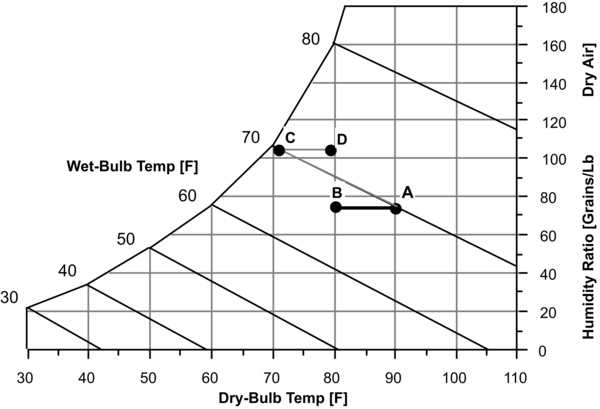
\includegraphics[width=0.9\textwidth, height=0.9\textheight, keepaspectratio=true]{media/image420.png}
\caption{Secondary Air Process -- Indirect Dry Coil Evap Cooler \protect \label{fig:secondary-air-process-indirect-dry-coil-evap}}
\end{figure}

The advantage of the dry coil heat exchanger is that the heat exchanger does not have the evaporation taking place on the outside of the tubes, thus no mineral deposits are left on the heat exchange surface to reduce the efficiency of the heat exchanger. The rigid media pads are designed to flush the mineral deposits to the sump, so the saturation efficiency of the pad stays relatively constant.

\subsubsection{Inputs}\label{inputs-2-013}

\paragraph{Field: Name}\label{field-name-2-012}

A unique identifying name for each evaporative cooler.

\paragraph{Field:Availability Schedule Name}\label{fieldavailability-schedule-name-1}

The name of a schedule which defines when the evaporative cooler is available. A schedule value of 0 indicates that the evaporative cooler is off for that time period. A schedule value greater than 0 indicates that the evaporative cooler can operate during the time period. If this field is blank, the schedule has values of 1 for all time periods.

\paragraph{Field: Direct Pad Area}\label{field-direct-pad-area-1}

The face area of the evaporative pad in m\(^{2}\). With the area and mass flow rate, the air velocity is calculated and is used to determine the saturation efficiency on the secondary side of the evaporative cooler. This field is autosizable.

\paragraph{Field: Direct Pad Depth}\label{field-direct-pad-depth-1}

The depth of the evaporative pad in meters. The pad depth is used to determine the saturation efficiency on the secondary side of the evaporative cooler. This field is autosizable.

\paragraph{Field: Recirculating Water Pump Power Consumption}\label{field-recirculating-water-pump-power-consumption-1}

This field is used to specify the power consumed by the evaporative cooler recirculating pump in Watts.

\paragraph{Field: Secondary Air Fan Flow Rate}\label{field-secondary-air-fan-flow-rate}

This field is used to specify the secondary air fan flow rate and is specified in m\(^{3}\)/sec.

\paragraph{Field: Secondary Fan Total Efficiency}\label{field-secondary-fan-total-efficiency}

This value is the overall efficiency of the fan, i.e., the ratio of the power delivered to the fluid to the electrical input power. It is the product of the motor efficiency and the impeller efficiency. The motor efficiency is the power delivered to the shaft divided by the electrical power input to the motor. The impeller efficiency is power delivered to the fluid (air) divided by the shaft power. The power delivered to the fluid is the mass flow rate of the air multiplied by the pressure rise divided by the air density. This input value must be between 0 and 1.

\paragraph{Field: Secondary Fan Delta Pressure}\label{field-secondary-fan-delta-pressure}

This field is used to specify the delta pressure across the secondary stage of the evaporative cooler in Pascals.

\paragraph{Field: Indirect Heat Exchanger Effectiveness}\label{field-indirect-heat-exchanger-effectiveness}

This field is used to specify the effectiveness of the indirect heat exchanger between the primary and secondary air flow.

\paragraph{Field: Primary Air Inlet Node Name}\label{field-primary-air-inlet-node-name-000}

The name of the evaporative cooler s primary air inlet node from the Air Loop Simulation. This is the air flow being cooled indirectly.

\paragraph{Field: Primary Air Outlet Node Name}\label{field-primary-air-outlet-node-name-000}

The name of the evaporative cooler s primary air outlet node from the Air Loop Simulation.

\paragraph{Field: Control Type}\label{field-control-type-1}

This input field is currently unused and can be left blank.

\paragraph{Field: Water Supply Storage Tank Name}\label{field-water-supply-storage-tank-name-2}

This field is optional. It is used to describe where the cooler obtains water used for evaporative cooling. If blank or omitted, then the cooler will obtain water directly from the mains. If the name of a WaterUse:Storage object is used here, then the cooler will obtain its water from that tank. If a tank is specified, the cooler will attempt to obtain all the water it uses from the tank. However if the tank cannot provide all the water the cooler needs, then the cooler will still operate and obtain the rest of the water it needs from the mains.

\paragraph{Field: Secondary Air Inlet Node Name}\label{field-secondary-air-inlet-node-name-000}

This field is optional. It is used to explicitly define an outdoor air node for the inlet for secondary air stream. Defining an outdoor air node here allows using the height-dependent model for outdoor air conditions.

And an IDF example showing how this object is specified:

\begin{lstlisting}

EvaporativeCooler:Indirect:CelDekPad,
  IndirectEvapCooler1,         !- Name
  FanAndCoilAvailSched,       !- Availability Schedule Name
  0.6,                                         !- Direct Pad Area {m2}
  0.2,                                         !- Direct Pad Depth {m}
  225.,                                       !- Recirculating Water Pump Power Consumption {W}
  1.0,                                         !- Secondary Air Fan Flow Rate {m3/s}
  0.7,                                         !- Secondary Fan Total Efficiency
  200.0,                                     !- Secondary Fan Delta Pressure {Pa}
  0.67,                                       !- Indirect Heat Exchanger Effectiveness
  EvapCoolerIndirectInletAirNode,   !- Primary Air Inlet Node Name
  EvapCoolerDirectInletAirNode,   !- Primary Air Outlet Node Name
  ,                                           !- Control Type
  ,                                               !- Water Supply Storage Tank Name
  Secondary side OA inlet node;   !- Secondary Air Inlet Node Name
\end{lstlisting}

\subsubsection{Outputs}\label{outputs-2-008}

The output variables that are available for the indirect dry evaporative cooler are shown below:

\begin{itemize}
\item
  HVAC,Average, Evaporative Cooler Wetbulb Effectiveness
\item
  HVAC,Average, Evaporative Cooler Total Stage Effectiveness
\item
  HVAC,Average, Evaporative Cooler Electric Power{[}W{]}
\item
  HVAC,Sum, Evaporative Cooler Electric Energy {[}J{]}
\item
  HVAC,Sum, Evaporative Cooler Water Volume{[}m3{]}
\item
  HVAC,Sum,Evaporative Cooler Mains Water Volume {[}m3{]}
\item
  HVAC,Sum,Evaporative Cooler Storage Tank Water Volume {[}m3{]}
\item
  HVAC,Sum,Evaporative Cooler Starved Water Volume {[}m3{]}
\item
  HVAC,Sum,Evaporative Cooler Starved Mains Water Volume {[}m3{]}
\end{itemize}

\paragraph{Evaporative Cooler Wetbulb Effectiveness}\label{evaporative-cooler-wetbulb-effectiveness}

The dry evaporation saturation efficiency is the saturation efficiency of the secondary or wet side air stream defined as the temperature change of the supply air divided by the difference between the outdoor dry-bulb and wet-bulb temperatures. In other words, it is a measure of the approach to the outdoor wet-bulb temperature.

\paragraph{Evaporative Cooler Total Stage Effectiveness}\label{evaporative-cooler-total-stage-effectiveness}

The total stage efficiency includes the sensible heat exchanger effectiveness of the heat exchanger in the supply air stream. It is the saturation efficiency multiplied by the heat exchanger effectiveness.

\paragraph{Evaporative Cooler Electric Power{[}W{]}}\label{evaporative-cooler-electric-powerw-2}

\paragraph{Evaporative Cooler Electric Energy {[}J{]}}\label{evaporative-cooler-electric-energy-j-2}

These output variables report the electric power and energy consumed by the secondary air fan and the sump pump.

\paragraph{Evaporative Cooler Water Volume{[}m3{]}}\label{evaporative-cooler-water-volumem3}

The water consumption is the water evaporated from the pad. This water consumption is only from the direct thermodynamics of water evaporation and does not include other sources of consumption such as drift or concentration blow down. This output variable appears when mains water is supplied to the cooler.

\paragraph{Evaporative Cooler Mains Water Volume {[}m3{]}}\label{evaporative-cooler-mains-water-volume-m3-2}

This is the source of the water consumed. This output variable appears when mains water is supplied to the cooler.

\paragraph{Evaporative Cooler Storage Tank Water Volume {[}m3{]}}\label{evaporative-cooler-storage-tank-water-volume-m3-2}

The water consumption is the water evaporated from the pad. This water consumption is only from the direct thermodynamics of water evaporation and does not include other sources of consumption such as drift or concentration blow down. This output variable appears when storage tank water is supplied to the cooler.

\paragraph{Evaporative Cooler Starved Water Volume {[}m3{]}}\label{evaporative-cooler-starved-water-volume-m3-2}

This is the water consumed by the evaporative cooler that could not accually be met by the storage tank. This output variable appears when storage tank water is supplied to the cooler.

\paragraph{Evaporative Cooler Starved Mains Water Volume {[}m3{]}}\label{evaporative-cooler-starved-mains-water-volume-m3-2}

This is the source (mains) of water consumed by the evaporative cooler that could not accually be met by the storage tank. This output variable appears when storage tank water is supplied to the cooler.

\subsection{EvaporativeCooler:Indirect:WetCoil}\label{evaporativecoolerindirectwetcoil}

The wetted coil evaporative cooler shown in the figure below, has water sprayed directly on the tubes of the heat exchanger where latent cooling takes place. The vaporization of the water on the outside of the heat exchanger tubes allows the simultaneous heat and mass transfer which removes heat from the supply air on the tube side. Then the moist secondary air is exhausted. The secondary air stream has its own fan.

\begin{figure}[hbtp] % fig 148
\centering
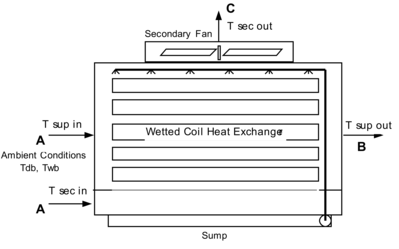
\includegraphics[width=0.9\textwidth, height=0.9\textheight, keepaspectratio=true]{media/image421.png}
\caption{Evaporative Cooler Indirect Wet Coil \protect \label{fig:evaporative-cooler-indirect-wet-coil}}
\end{figure}

The process that the secondary air goes through, A to C on the following figure, is a path of simultaneous heat and mass transfer, but it does not follow a line of constant enthalpy as in the direct stage. The process is not adiabatic due to the heat gain from the supply air flowing through the tubes of the heat exchanger.

\begin{figure}[hbtp] % fig 149
\centering
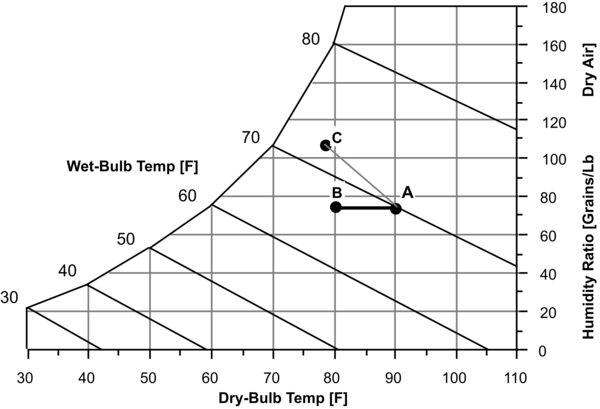
\includegraphics[width=0.9\textwidth, height=0.9\textheight, keepaspectratio=true]{media/image422.png}
\caption{Secondary Air Process Indirect Wet Coil Evap Cooler \protect \label{fig:secondary-air-process-indirect-wet-coil-evap}}
\end{figure}

The wet coil heat exchanger can have a higher stage efficiency than the dry coil due to a higher heat transfer rate on the outside of the heat exchanger tubes. Over the operating lifetime of the heat exchanger, the vaporization taking place on the heat exchange surface can leave mineral deposits which will decrease the effectiveness of the heat exchanger.

\subsubsection{Inputs}\label{inputs-3-012}

\paragraph{Field: Name}\label{field-name-3-011}

A unique identifying name for each evaporative cooler.

\paragraph{Field:Availability Schedule Name}\label{fieldavailability-schedule-name-2}

The name of a schedule which defines when the evaporative cooler is available. A schedule value of 0 indicates that the evaporative cooler is off for that time period. A schedule value greater than 0 indicates that the evaporative cooler can operate during the time period. If this field is blank, the schedule has values of 1 for all time periods.

\paragraph{Field: Coil Maximum Efficiency}\label{field-coil-maximum-efficiency}

The maximum efficiency of the stage is a combination of the efficiency due to the simultaneous heat and mass transfer on the outside of the tube and the efficiency of the heat exchanger. This value can be higher than the dry coil overall efficiency since the convective coefficients on the outside of the tube are larger.

\paragraph{Field: Coil Flow Ratio}\label{field-coil-flow-ratio}

The Coil Flow Ratio is determined from performance data. The Coil Flow Ratio tells how quickly the efficiency of the stage would decrease with a mismatch of the supply and secondary flows.

\paragraph{Field: Recirculating Water Pump Power Consumption}\label{field-recirculating-water-pump-power-consumption-2}

This field is used to specify the power consumed by the evaporative cooler recirculating pump in Watts.

\paragraph{Field: Secondary Air Fan Flow Rate}\label{field-secondary-air-fan-flow-rate-1}

This field is used to specify the secondary air fan flow rate and is specified in m\(^{3}\)/sec.

\paragraph{Field: Secondary Air Fan Total Efficiency}\label{field-secondary-air-fan-total-efficiency}

This value is the overall efficiency of the fan, i.e., the ratio of the power delivered to the fluid to the electrical input power. It is the product of the motor efficiency and the impeller efficiency. The motor efficiency is the power delivered to the shaft divided by the electrical power input to the motor. The impeller efficiency is power delivered to the fluid (air) divided by the shaft power. The power delivered to the fluid is the mass flow rate of the air multiplied by the pressure rise divided by the air density. This input value must be between 0 and 1..

\paragraph{Field: Secondary Air Fan Delta Pressure}\label{field-secondary-air-fan-delta-pressure}

This field is used to specify the delta pressure across the secondary stage of the evaporative cooler in Pascals.

\paragraph{Field: Primary Air Inlet Node Name}\label{field-primary-air-inlet-node-name-1}

The name of the evaporative cooler air inlet from the Air Loop Simulation.

\paragraph{Field: Primary Air Outlet Node Name}\label{field-primary-air-outlet-node-name-1}

The name of the evaporative cooler air outlet from the Air Loop Simulation.

\paragraph{Field: Control Type}\label{field-control-type-2}

This input field is currently unused and can be left blank.

\paragraph{Field: Water Supply Storage Tank Name}\label{field-water-supply-storage-tank-name-3}

This field is optional. It is used to describe where the cooler obtains water used for evaporative cooling. If blank or omitted, then the cooler will obtain water directly from the mains. If the name of a WaterUse:Storage object is used here, then the cooler will obtain its water from that tank. If a tank is specified, the cooler will attempt to obtain all the water it uses from the tank. However if the tank cannot provide all the water the cooler needs, then the cooler will still operate and obtain the rest of the water it needs from the mains.

\paragraph{Field: Secondary Air Inlet Node Name}\label{field-secondary-air-inlet-node-name-1-000}

This field is optional. It is used to explicitly define an outdoor air node for the inlet for secondary air stream. Defining an outdoor air node here allows using the height-dependent model for outdoor air conditions.

\paragraph{Field: Drift Loss Fraction}\label{field-drift-loss-fraction-1}

This field is optional and can be used to model additional water consumed by the cooler from drift. Drift is water that leaves the cooling media as droplets and does not evaporate into the process air stream. For example, water may get blown off the evaporative media by winds and escape the air system. The value entered here is a simple fraction of the water consumed by the cooler for normal process evaporation. The amount of drift is this fraction times the water evaporated for the normal cooling process. This field can be left blank and then there will be no added water consumption from drift.

\paragraph{Field: Blowdown Concentration Ratio}\label{field-blowdown-concentration-ratio-1-000}

This field is optional and can be used to model additional water consumed by the cooler from blowdown. Blowdown is water that is intentionally drained from the cooler s sump to offset the build up of solids in the water that would otherwise occur because of evaporation. The value entered here is dimensionless. It can be characterized as the ratio of solids in the blowdown water to solids in the make up water. Typical values are 3 to 5. The default is 3.0.

And an IDF example showing how this object is specified:

\begin{lstlisting}

EvaporativeCooler:Indirect:WetCoil,
  IndirectEvapCooler1,         !- Name
  FanAndCoilAvailSched,       !- Availability Schedule Name
  0.8,                                         !- Coil Maximum Efficiency
  0.16,                                       !- Coil Flow Ratio
  225.,                                       !- Recirculating Water Pump Power Consumption {W}
  1.0,                                         !- Secondary Air Fan Flow Rate {m3/s}
  0.7,                                         !- Secondary Air Fan Total Efficiency
  200.0,                                     !- Secondary Air Fan Delta Pressure {Pa}
  EvapCoolerIndirectInletAirNode,   !- Primary Air Inlet Node Name
  EvapCoolerDirectInletAirNode,   !- Primary Air Outlet Node Name
  ,                                               !- Control Type
  ,                                               !- Water Supply Storage Tank Name
  Secondary side OA inlet node;   !- Secondary Air Inlet Node Name
\end{lstlisting}

\subsubsection{Outputs}\label{outputs-3-006}

The output variables that are available for the wet indirect evaporative cooler are shown below:

\begin{itemize}
\item
  HVAC,Average, Evaporative Cooler Total Stage Effectiveness
\item
  HVAC,Average, Evaporative Cooler Electric Power{[}W{]}
\item
  HVAC,Sum, Evaporative Cooler Electric Energy {[}J{]}
\item
  HVAC,Sum, Evaporative Cooler Water Volume{[}m3{]}
\item
  HVAC,Sum,Evaporative Cooler Mains Water Volume {[}m3{]}
\item
  HVAC,Sum,Evaporative Cooler Storage Tank Water Volume {[}m3{]}
\item
  HVAC,Sum,Evaporative Cooler Starved Water Volume {[}m3{]}
\item
  HVAC,Sum,Evaporative Cooler Starved Mains Water Volume {[}m3{]}
\end{itemize}

\paragraph{Evaporative Cooler Total Stage Effectiveness {[]}}\label{evaporative-cooler-total-stage-effectiveness-1}

The Total Stage Efficiency is defined as the temperature change of the supply air divided by the difference between the outdoor dry-bulb and wet-bulb temperatures, including the effect of the reduction in flow because of the secondary air stream. In other words, it is a measure of the approach to the outdoor wet-bulb temperature.

\paragraph{Evaporative Cooler Electric Power {[}W{]}}\label{evaporative-cooler-electric-power-w}

\paragraph{Evaporative Cooler Electric Energy {[}J{]}}\label{evaporative-cooler-electric-energy-j-3}

These output variables report the electric power and energy that are consumed by the secondary air fan and the sump pump.

\paragraph{Evaporative Cooler Water Volume {[}m3{]}}\label{evaporative-cooler-water-volume-m3-2}

The water consumption is the water evaporated from the pad. This water consumption is only from the direct thermodynamics of water evaporation and does not include other sources of consumption such as drift or concentration blow down. This output variable appears when mains water is supplied to the cooler.

\paragraph{Evaporative Cooler Mains Water Volume {[}m3{]}}\label{evaporative-cooler-mains-water-volume-m3-3}

This is the source of the water consumed. This output variable appears when mains water is supplied to the cooler.

\paragraph{Evaporative Cooler Storage Tank Water Volume {[}m3{]}}\label{evaporative-cooler-storage-tank-water-volume-m3-3}

The water consumption is the water evaporated from the pad. This water consumption is only from the direct thermodynamics of water evaporation and does not include other sources of consumption such as drift or concentration blow down. This output variable appears when storage tank water is supplied to the cooler.

\paragraph{Evaporative Cooler Starved Water Volume {[}m3{]}}\label{evaporative-cooler-starved-water-volume-m3-3}

This is the water consumed by the evaporative cooler that could not accually be met by the storage tank. This output variable appears when storage tank water is supplied to the cooler.

\paragraph{Evaporative Cooler Starved Mains Water Volume {[}m3{]}}\label{evaporative-cooler-starved-mains-water-volume-m3-3}

This is the source (mains) of water consumed by the evaporative cooler that could not accually be met by the storage tank. This output variable appears when storage tank water is supplied to the cooler.

\subsection{EvaporativeCooler:Indirect:ResearchSpecial}\label{evaporativecoolerindirectresearchspecial}

This cooler is similar in principal to the EvaporativeCooler:Indirect:CelDekPad and EvaporativeCooler:Indirect:WetCoil (see Figure~\ref{fig:secondary-air-process-indirect-dry-coil-evap}, Figure~\ref{fig:evaporative-cooler-indirect-wet-coil}, and Figure~\ref{fig:secondary-air-process-indirect-wet-coil-evap}). The model differs in that it gives the user more flexibility to specify the source of secondary air. The cooler effectiveness with respect to wetbulb depression is allowed to go beyond 1.0. Using the ResearchSpecial input object also allows the cooler to control the amount of cooling based on node setpoints (controlled by SetpointManagers). This avoid problems from over cooling when conditions are such that loads are low and cooling power is high. Fan power is assumed to vary linearly when the cooler is operating at less than full capacity.

The indirect evaporative cooler research special calculation procedure allows accounting for dry and wet effectiveness value variation with flow fraction. Two effectiveness modifier curves are included as optional user inputs for this purpose. Effectiveness modifier curves operate on the design dry and wet effectiveness values. The flow fraction is calculated as a ratio of the sum of current primary and secondary air flow rates to the sum of the design flow rates. Model also accounts for fan and recirculation water pump power variation with secondary air flow rates using pump power modifying curve. The fan power is calculated by multiplying the design fan power using fan power modify curve value evaluated at current secondary air flow fraction. Similarly, recirculating pump power is is calculated by multiplying the design pump power by pump power modifier curve value evaluated at current secondary air flow fraction. If the secondary air fan and recirculating pump power modifier curves are not specified, then fan and pump power are assumed to vary linearly with part load fraction.

\subsubsection{Inputs}\label{inputs-4-011}

\paragraph{Field: Name}\label{field-name-4-010}

A unique identifying name for each cooler.

\paragraph{Field: Availability Schedule Name}\label{field-availability-schedule-name-1-004}

The name of a schedule that defines when the evaporative cooler is available. A schedule value of 0 indicates that the evaporative cooler is off for that time period. A schedule value greater than 0 indicates that the evaporative cooler can operate during the time period. If this field is blank, the schedule has values of 1 for all time periods.

\paragraph{Field: Cooler Wetbulb Design Effectiveness}\label{field-cooler-wetbulb-design-effectiveness}

This field specifies the design effectiveness that is applied to the wetbulb depression to determine the conditions leaving the cooler. This effectiveness is a complicated function of the efficiency with which heat and mass are transferred on the secondary side and the efficiency of heat exchange between the secondary and primary flows. The model assumes that the effectiveness a function of flow fraction. The flow fraction is the ratio of the sum of primary air and secondary air current flow rates and the sum of the primary air and secondary air design flow rates.

\paragraph{Field: Wet Bulb Effectiveness Flow Ratio Modifier Curve Name}\label{field-wet-bulb-effectiveness-flow-ratio-modifier-curve-name}

This curve modifies the wet bulb effectiveness design value specified the previous field by multiplying the value by the result of this curve. The modifying curve is a function of flow fraction, which is the ratio of the sum of the primary and secondary flow rates divided by the sum of the design flow rates. If this input field is left blank, the effectiveness is assumed to be constant. Any curve or table with one independent variable can be used. Any curve or table with one independent variable can be used: Curve:Linear, Curve:Quadratic, Curve:Cubic, Curve:Quartic, Curve:Exponent, Curve:ExponentialSkewNormal, Curve:Sigmoid, Curve:RectuangularHyperbola1, Curve:RectangularHyperbola2, Curve:ExponentialDecay, Curve:DoubleExponentialDecay, and Table:OneIndependentVariable.

\paragraph{Field: Cooler Drybulb Design Effectiveness}\label{field-cooler-drybulb-design-effectiveness}

This input value is dry bulb design effectiveness of the evaporative cooler. This is the nominal design dry blub effectiveness with respect to dry bulb temperature difference, i.e., dry operation and at design air flow rates, and no water evaporation or spraying on the secondary side.

\paragraph{Field Drybulb Effectiveness Flow Ratio Modifier Curve Name}\label{field-drybulb-effectiveness-flow-ratio-modifier-curve-name}

This this curve modifies the drybulb effectiveness in the previous field (eff\_db\_design) by multiplying the design effectiveness value by the result of this curve. The curve is evaluated flow fraction as independent variable. The flow fraction is the ratio of sum of the primary and secondary flow rates divided by the sum of the design flow rates. If this input field is left blank, the effectiveness is assumed to be constant. Any curve or table with one independent variable can be used: Curve:Linear, Curve:Quadratic, Curve:Cubic, Curve:Quartic, Curve:Exponent, Curve:ExponentialSkewNormal, Curve:Sigmoid, Curve:RectuangularHyperbola1, Curve:RectangularHyperbola2, Curve:ExponentialDecay, Curve:DoubleExponentialDecay, and Table:OneIndependentVariable.

\paragraph{Field: Recirculating Water Pump Design Power}\label{field-recirculating-water-pump-design-power}

This numeric input field is the recirculating pump electric power at Secondary Design Air Flow Rate in W. This is the nominal design pump power water recirculation and spray for evaporation at design secondary air flow rates and cooler design effectiveness. This input field is autosizable.

\paragraph{Field: Water Pump Power Sizing Factor}\label{field-water-pump-power-sizing-factor-1}

This numeric input field value is recirculating water pump sizing factor in W/(m3/s). This field is used when the previous field is set to autosize. The pump design electric power is scaled with Secondary Design Air Flow Rate. Average Pump Power sizing factor was estimated from pump power and secondary air design flow rates inputs from energyplus example files is about 90.0 {[}W/(m3/s){]} ( = 90.0 \textasciitilde{} Pump Power / Secondary Air Design Flow Rate). The factor ranges from 55.0 to 150.0 {[}W/(m3/s){]}.

\paragraph{Field: Water Pump Power Modifier Curve Name}\label{field-water-pump-power-modifier-curve-name-1}

This alpha input field is the name of a dimensionless normalized pump power modifying curve. This curve modifies the pump electric power in the previous field by multiplying the design power by the result of this curve. The normalized curve is a function of the secondary side flow fraction as independent variable. The curve shall yield a value of 1.0 at a flow fraction of 1.0. The flow fraction is the secondary air flow rate during operation divided by Secondary Design Air Flow Rate. If this input field is left blank, the pump power is assumed to be constant. Any curve or table with one independent variable can be used: Curve:Linear, Curve:Quadratic, Curve:Cubic, Curve:Quartic, Curve:Exponent, Curve:ExponentialSkewNormal, Curve:Sigmoid, Curve:RectuangularHyperbola1, Curve:RectangularHyperbola2, Curve:ExponentialDecay, Curve:DoubleExponentialDecay, and Table:OneIndependentVariable.

\paragraph{Field: Secondary Air Design Flow Rate}\label{field-secondary-air-design-flow-rate}

This field is used to specify the secondary air fan flow rate and is specified in m\(^{3}\)/s. This flow rate would typically be similar in magnitude to the flow through the primary side. This field can be autosized. When it is autosized, the program detects if the component is in the main air loop or on an outdoor air path. If it is on the main air loop, then the flow rate is set to the AirLoopHVAC system s design supply air flow rate (which is the maximum required for heating and cooling). If it is on the outdoor air path, then the flow rate is set to the larger of either the design minimum outdoor air flow rate or one-half of the main air loop design flow rate. The flow rate is used to determine parasitic fan energy and cooler effectiveness. The flow rate (and fan power) is effectively reduced by cycling when the amount of cooling needs to be restricted for control purpose. This field can be autosized. When this input is autosized, the program calculates by scaling the Primary Air Design Flow Rate using secondary air scaling factor specified in the input field below.

\paragraph{Field: Secondary Air Flow Scaling Factor}\label{field-secondary-air-flow-scaling-factor}

This numeric input field is used to scale the secondary air design flow rate and it is dimensionless. This field is used when the previous field is set to autosize. The Primary Design Air Flow Rate is scaled using this factor to calculate the secondary design air flow rate.

\paragraph{Field: Secondary Air Fan Design Power}\label{field-secondary-air-fan-design-power}

This numeric input field is the fan electric power at Secondary Design Air Flow Rate. This is the nominal design electric power at full speed of the secondary air fan. This input field is autosizable.

\paragraph{Field: Secondary Air Fan Sizing Specific Power}\label{field-secondary-air-fan-sizing-specific-power}

This input field value is secondary air fan sizing specific power in W/(m3/s). This field is used when the previous field is set to autosize. The fan power is scaled with Secondary Design Air Flow Rate.

\paragraph{Field: Secondary Air Fan Power Modifier Curve Name}\label{field-secondary-air-fan-power-modifier-curve-name}

This input field is the name of a dimensionless normalized curve. The normalized curve modifies the design secondary air fan power in the previous field by multiplying the value by the result of this curve. The normalized curve is a function of the secondary side flow fraction as independent variable. The curve shall yield a value of 1.0 at a flow fraction of 1.0. The flow fraction is the secondary air flow rate during operation divided by Secondary Design Air Flow Rate. If this input field is left blank, the fan power is assumed to be constant. Any curve or table with one independent variable can be used: Curve:Linear, Curve:Quadratic, Curve:Cubic, Curve:Quartic, Curve:Exponent, Curve:ExponentialSkewNormal, Curve:Sigmoid, Curve:RectuangularHyperbola1, Curve:RectangularHyperbola2, Curve:ExponentialDecay, Curve:DoubleExponentialDecay, and Table:OneIndependentVariable.

\paragraph{Field: Primary Air Inlet Node Name}\label{field-primary-air-inlet-node-name-2}

The name of the air inlet node for the primary air flow path through the cooler.

\paragraph{Field: Primary Air Outlet Node Name}\label{field-primary-air-outlet-node-name-2}

The name of the air outlet node for the primary air flow path through the cooler.

\paragraph{Field:Primary Design Air Flow Rate}\label{fieldprimary-design-air-flow-rate-1}

This numeric input field is the primary air design air flow rate in m3/s. This input field is autosizable. If the evaporative cooler is on main air loop branch, the design flow rate is the same as branch design flow rate, or else if it is on outdoor air system it will be the maximum of the the outdoor air design flow rate and the half of the primary air flow rate on the main air loop branch.

\paragraph{Field: Dewpoint Effectiveness Factor}\label{field-dewpoint-effectiveness-factor}

This field specifies an effectiveness that is applied to the dewpoint depression to determine a bound for the conditions leaving the cooler. The model uses the warmer of the two temperatures determined from wetbulb depression and dewpoint depression.

\paragraph{Field: Secondary Air Inlet Node Name}\label{field-secondary-air-inlet-node-name-2}

This field specifies the name of the node providing air to the secondary/wet side of the cooler. Typically this node could appear in an outdoor air node list or be part of an air system loop.

\paragraph{Field: Secondary Air Outlet Node Name}\label{field-secondary-air-outlet-node-name}

This alpha input field is the name of the secondary air side outlet node.

\paragraph{Field: Sensor Node Name}\label{field-sensor-node-name-1}

This field specifies the name of a node that will provide system air temperature setpoint information. A separate SetpointManager object should be setup to update this node.

\paragraph{Field: Relief Air Inlet Node Name}\label{field-relief-air-inlet-node-name}

This field is optional, but can be used to feed two sources of secondary air into the wet side of the cooler. Typical use is to run the air system relief air into the system. The model first uses all of the air flow available from this node and then adds the air flow from the secondary air inlet node to make up the total defined by Secondary air Fan Flow Rate.

\paragraph{Field: Water Supply Storage Tank Name}\label{field-water-supply-storage-tank-name-4}

This field is optional. It is used to describe where the cooler obtains water used for evaporative cooling. If blank or omitted, then the cooler will obtain water directly from the mains. If the name of a WaterUse:Storage object is used here, then the cooler will obtain its water from that tank. If a tank is specified, the cooler will attempt to obtain all the water it uses from the tank. However, if the tank cannot provide all the water the cooler needs, then the cooler will still operate and obtain the rest of the water it needs from the mains.

\paragraph{Field: Drift Loss Fraction}\label{field-drift-loss-fraction-2}

This field is optional and can be used to model additional water consumed by the cooler from drift. Drift is water that leaves the cooling media as droplets and does not evaporate into the process air stream. For example, water may get blown off the evaporative media by winds and escape the air system. The value entered here is a simple fraction of the water consumed by the cooler for normal process evaporation. The amount of drift is this fraction times the water evaporated for the normal cooling process. This field can be left blank and then there will be no added water consumption from drift.

\paragraph{Field: Blowdown Concentration Ratio}\label{field-blowdown-concentration-ratio-2-000}

This field is optional and can be used to model additional water consumed by the cooler from blowdown. Blowdown is water that is intentionally drained from the cooler s sump to offset the build up of solids in the water that would otherwise occur because of evaporation. The value entered here is dimensionless. It can be characterized as the ratio of solids in the blowdown water to solids in the make up water. Typical values are 3 to 5. The default is 3.0.

\paragraph{Field: Evaporative Operation Minimum Limit Drybulb Temperature}\label{field-evaporative-operation-minimum-limit-drybulb-temperature}

This input field value defines the secondary air inlet node drybulb temperature limits in degree Celsius. When the secondary side entering air dry bulb temperature drops below this limit, then the evaporative cooler operation mode changes to dry heat exchanger. Users specify their own limits. If this field is left blank, then there is no drybulb temperature lower limit for evaporative cooler operation. If operating range control is desired then this input field and the next two input fields should be specified or all the three should be left blank or left out. If no minimum drybulb temperature limit is required while there are maximum drybulb and wetbulb temperature limits then specify very low temperature limit value (e.g., -99.0 C).

\paragraph{Field: Evaporative Operation Maximum Limit Wetbulb Temperature}\label{field-evaporative-operation-maximum-limit-wetbulb-temperature-1}

This input field value defines the secondary air inlet node wetbulb temperature limits in degree Celsius. When the secondary side entering air wet bulb temperature exceeds this limit, then the evaporative cooler is turns off and does not attempt to do any cooling. If this field is left blank, then there is no wetbulb temperature maximum limit for evaporative cooler wet operation mode. If no upper wetbulb temperature limits is desired while there are minimum drybulb and maximum drybulb upper temperature limits then then specify very high maximum wetbulb temperature limit value (e.g.~99.0 C).

\paragraph{Field: Evaporative Operation Maximum Limit Drybulb Temperature}\label{field-evaporative-operation-maximum-limit-drybulb-temperature-1}

This input field value defines the secondary air inlet node drybulb temperature limits in degree Celsius. When the secondary side entering air drybulb temperature exceeds this limit, the evaporative cooler will not run in dry operation mode or may be turned off depending on its wetbulb temperature. If this field is left blank, then there is no drybulb temperature maximum limit for evaporative cooler dry operation mode.

If no drybulb temperature limit is desired while there are minimum drybulb and maximum wetbulb temperature limits then specify very high maximum drybulb temperature limit value (e.g.~99.0 C).

An IDF example is shown below:

\begin{lstlisting}

EvaporativeCooler:Indirect:ResearchSpecial,
  DataC_IndirectEvapCooler,     !- Name
  ALWAYS_ON,                    !- Availability Schedule Name
  0.75,                         !- Cooler Wetbulb Design Effectiveness
  ,              !- Wetbulb Effectiveness Flow Ratio Modifier Curve Name
  ,                          !- Cooler Drybulb Design Effectiveness
  ,              !- Drybulb Effectiveness Flow Ratio Modifier Curve Name
  autosize,                     !- Recirculating Water Pump Power
  autosize,                     !- Secondary Air Design Flow Rate  
  1.0,                          !- Secondary Air Flow Scaling Factor

  autosize,                     !- Secondary Air Fan Design Power
  800.0,                        !- Secondary Air Fan Sizing Specific Power W
  ,               !- Secondary Air Fan Power Modifier Curve Name
  Return Air Node,              !- Primary Air Inlet Node Name
  IndEC Outlet Node,            !- Primary Air Outlet Node Name
  autosize,                     !- Primary Design Air Flow Rate  
  0.9 ,                         !- Dewpoint Effectiveness Factor
  IndEC OA Air Inlet Node,      !- Secondary Air Inlet Node Name
  IndEC OA Air Outlet Node,     !- Secondary Air Outlet Node Name
  IndEC Outlet Node,            !- Sensor Node Name
  ,                             !- Relief Air Inlet Node Name
  ,                             !- Water Supply Storage Tank Name
  0.0,                          !- Drift Loss Fraction
  ;                             !- Blowdown Concentration Ratio
\end{lstlisting}

\subsubsection{Outputs}\label{outputs-4-004}

The output variables that are available for the EvaporativeCooler:Indirect:ResearchSpecial object are shown below:

\begin{itemize}
\item
  HVAC,Average,Evaporative Cooler Total Stage Effectiveness
\item
  HVAC,Average,Evaporative Cooler Part Load Ratio
\item
  HVAC,Average,Evaporative Cooler Dewpoint Bound Status
\item
  HVAC,Average,Evaporative Cooler Operating Mode Satus {[]}
\item
  HVAC,Sum,Evaporative Cooler Electric Energy {[}J{]}
\item
  HVAC,Average,Evaporative Cooler Electric Power {[}W{]}
\item
  HVAC,Sum,Evaporative Cooler Storage Tank Water Volume {[}m3{]}
\item
  HVAC,Sum,Evaporative Cooler Starved Water Volume {[}m3{]}
\item
  HVAC,Sum,Evaporative Cooler Starved Mains Water Volume {[}m3{]}
\end{itemize}

\paragraph{Evaporative Cooler Total Stage Effectiveness {[]}}\label{evaporative-cooler-total-stage-effectiveness-2}

The Total Stage Efficiency is defined as the temperature change of the supply air divided by the difference between the primary air entering dry-bulb temperature and the secondary air enterig wet-bulb temperature for wet operating mode or the the difference between the primary air entering dry-bulb temperature and the secondary air enterig dry-bulb temperature for dry operating mode, including the effect of the reduction in flow because of the secondary air stream. In other words, it is a measure of the approach to the secondary air wet-bulb temperature for wet operating mode, or it is a measure of the approach to the secondary air entering dry-bulb temperature for dry operating mode.

\paragraph{Evaporative Cooler Operating Mode Status {[]}}\label{evaporative-cooler-operating-mode-status}

This output variable provides the operating modes or status of the indirect evaporative cooler. This output variable can have status indicator integer value of 0, 1, or 2 representing Off, Dry and Wet operating modes, respectively.

\paragraph{Evaporative Cooler Part Load Ratio {[]}}\label{evaporative-cooler-part-load-ratio}

This output variable provides the part load fraction of the indirect cooler. The ResearchSpecial cooler model is able to modulate to meet a temperature set point to avoid over cooling. This output variable is the fraction formed by the ratio of the capacity needed over the maximum cooling capacity available. A value of 1.0 corresponds to full capacity cooling.

\paragraph{Evaporative Cooler Dewpoint Bound Status {[]}}\label{evaporative-cooler-dewpoint-bound-status}

This output variable is a flag that indicates if the modeling was based on dewpoint effectivenss rather than wetbulb effectiveness The ResearchSpecial model is usually based on wet-bulb approach, but since values in excess of 1.0 are allowed, there is a secondary constraint imposed by dewpoint. If the dewpoint effectiveness was applied, then this flag variable will have the value 1.0, otherwise it is 0.0.

\paragraph{Evaporative Cooler Electric Power {[}W{]}}\label{evaporative-cooler-electric-power-w-1}

\paragraph{Evaporative Cooler Electric Energy {[}J{]}}\label{evaporative-cooler-electric-energy-j-4}

These output variables report the electric power and energy that are consumed by the secondary air fan and the sump pump.

\paragraph{Evaporative Cooler Water Volume {[}m3{]}}\label{evaporative-cooler-water-volume-m3-3}

The water consumption is the water evaporated from the pad. This water consumption is only from the direct thermodynamics of water evaporation and does not include other sources of consumption such as drift or concentration blow down. This output variable appears when mains water is supplied to the cooler.

\paragraph{Evaporative Cooler Mains Water Volume {[}m3{]}}\label{evaporative-cooler-mains-water-volume-m3-4}

This is the source of the water consumed. This output variable appears when mains water is supplied to the cooler.

\paragraph{Evaporative Cooler Storage Tank Water Volume {[}m3{]}}\label{evaporative-cooler-storage-tank-water-volume-m3-4}

The water consumption is the water evaporated from the pad. This water consumption is only from the direct thermodynamics of water evaporation and does not include other sources of consumption such as drift or concentration blow down. This output variable appears when storage tank water is supplied to the cooler.

\paragraph{Evaporative Cooler Starved Water Volume {[}m3{]}}\label{evaporative-cooler-starved-water-volume-m3-4}

This is the water consumed by the evaporative cooler that could not accually be met by the storage tank. This output variable appears when storage tank water is supplied to the cooler.

\paragraph{Evaporative Cooler Starved Mains Water Volume {[}m3{]}}\label{evaporative-cooler-starved-mains-water-volume-m3-4}

This is the source (mains) of water consumed by the evaporative cooler that could not accually be met by the storage tank. This output variable appears when storage tank water is supplied to the cooler.
